%!TEX program = xelatex
\documentclass[12pt, a4paper]{article}

\usepackage[dvipsnames]{xcolor}

\usepackage{fancyhdr}
\usepackage{extramarks}
\usepackage{amsmath}
\usepackage{empheq}
\usepackage{amsthm}
\usepackage{amsfonts}
\usepackage{tikz}
\usepackage{tikz-3dplot}
\usepackage[plain]{algorithm}
\usepackage{algpseudocode}

\usepackage{ctex}
\usepackage{upgreek}
\usepackage{indentfirst}
\usepackage{wrapfig}
\usepackage{subfigure}
\usepackage{pgfplots}
\usepgfplotslibrary{patchplots}
\usepgfplotslibrary{colormaps}
\usepgfplotslibrary{colorbrewer}
\pgfplotsset{compat=1.18}
\usetikzlibrary{automata,positioning,shapes.geometric,arrows.meta,patterns,calc}
\numberwithin{equation}{section}
\CTEXoptions[today=old]

%
% Basic Document Settings
%

\topmargin=-0.25in
\evensidemargin=0in
\oddsidemargin=0in
\textwidth=6.5in
\textheight=9.2in
\headsep=0.25in

\linespread{1.1}

\pagestyle{fancy}
\lhead{\hmwkAuthorName}
\chead{\hmwkClass : \hmwkTitle}
\rhead{\firstxmark}
\lfoot{\lastxmark}
\cfoot{\thepage}

\renewcommand\headrulewidth{0.4pt}
\renewcommand\footrulewidth{0.4pt}

\setlength{\parindent}{2em}  % 2em代表首行缩进两个字符

%
% Create Problem Sections
%

\newcommand{\enterProblemHeader}[1]{
    \nobreak\extramarks{}{Problem \arabic{#1} continued on next page\ldots}\nobreak{}
    \nobreak\extramarks{Problem \arabic{#1} (continued)}{Problem \arabic{#1} continued on next page\ldots}\nobreak{}
}

\newcommand{\exitProblemHeader}[1]{
    \nobreak\extramarks{Problem \arabic{#1} (continued)}{Problem \arabic{#1} continued on next page\ldots}\nobreak{}
    \stepcounter{#1}
    \nobreak\extramarks{Problem \arabic{#1}}{}\nobreak{}
}

% \setcounter{secnumdepth}{0}
\newcounter{partCounter}
\newcounter{homeworkProblemCounter}
\setcounter{homeworkProblemCounter}{0}
% \nobreak\extramarks{Problem \arabic{homeworkProblemCounter}}{}\nobreak{}

%
% Homework Problem Environment
%
% This environment takes an optional argument. When given, it will adjust the
% problem counter. This is useful for when the problems given for your
% assignment aren't sequential. See the last 3 problems of this template for an
% example.
%
\newenvironment{homeworkProblem}[1][-1]{
    \ifnum#1>0
        \setcounter{homeworkProblemCounter}{#1}
    \fi
    \section{Problem \arabic{homeworkProblemCounter}}
    \setcounter{partCounter}{1}
    \enterProblemHeader{homeworkProblemCounter}
}{
    \exitProblemHeader{homeworkProblemCounter}
}

%
% Homework Details
%   - Title
%   - Due date
%   - Class
%   - Section/Time
%   - Instructor
%   - Author
%

\newcommand{\hmwkTitle}{Multiple Integral}
\newcommand{\hmwkClass}{Advanced Mathematics}
\newcommand{\hmwkClassTime}{}
\newcommand{\myUniversiy}{Wuhan University}
\newcommand{\hmwkAuthorName}{\textbf{Lai Wei}}

%
% Title Page
%

\title{
    \vspace{2in}
    \textmd{\textbf{\hmwkClass:\ \hmwkTitle}}\\
    \vspace{0.4in}
    \large{\textit{\myUniversiy}}
    \vspace{3in}
}

\author{\hmwkAuthorName}
\date{\today}

\renewcommand{\part}[1]{\textbf{\large Part \Alph{partCounter}}\stepcounter{partCounter}\\}

%
% Various Helper Commands
%

% Useful for algorithms
\newcommand{\alg}[1]{\textsc{\bfseries \footnotesize #1}}

% % For derivatives
% \newcommand{\deriv}[1]{\frac{\mathrm{d}}{\mathrm{d}x} (#1)}

% For partial derivatives
% \newcommand{\pderiv}[2]{\frac{\partial}{\partial #1} (#2)}

% Integral dx
\newcommand{\dx}{\mathrm{d}x}

% Alias for the Solution section header
\newcommand{\solution}{\textbf{\large Solution}}

% Probability commands: Expectation, Variance, Covariance, Bias
\newcommand{\E}{\mathrm{E}}
\newcommand{\Var}{\mathrm{Var}}
\newcommand{\Cov}{\mathrm{Cov}}
\newcommand{\Bias}{\mathrm{Bias}}

% 我的newcommand
\newcommand{\degree}{^{\circ}}
\newcommand{\arrow}{-{Stealth[length=4mm,width=2mm]}}
\newcommand{\rmd}{\mathrm{d}}
\newcommand{\deriv}[2]{\frac{\rmd #1}{\rmd #2}}
\renewcommand{\parallel}{\mathrel{/\mskip-2.5mu/}}
\newcommand{\pderiv}[2]{\frac{\partial #1}{\partial #2}}
\newcommand{\parallelogram}{
	\mathord
    {\text
        {
			\tikz[baseline]
			\draw (0,.1ex) -- (.8em,.1ex) -- (1em,1.6ex) -- (.2em,1.6ex) -- cycle;
        }
    }
}

\begin{document}

\maketitle

\pagebreak

% 设置页码格式是罗马数字
\pagenumbering{roman}

% 生成目录
\tableofcontents

\pagebreak

% 设置页码格式是阿拉伯数字
\pagenumbering{arabic}

\pagebreak

\section{二重积分的概念与性质}

\subsection{二重积分的概念}

\subsubsection{定义}

    设\(f\left(x,y\right)\)是有界闭区域\(D \)上的有界函数。将闭区域\(D \)任意分成\(n \)个小闭区域
    
    $$
        \Delta \sigma_1, \Delta \sigma_2, \cdots, \Delta \sigma_n
    $$

    其中\(\Delta \sigma_i \)表示第\(i \)个小闭区域,也表示它的面积。
    在每个\(\Delta \sigma_i\)上任取一点\(\left(\xi_i, \eta_i\right)\),
    作乘积\(f\left(\xi_i, \eta_i \right)\Delta \sigma_i\)(\(i = 1, 2, \cdots n \)),
    并作和\({\displaystyle \sum_{i=1}^{n }f\left(\xi_i, \eta_i \right)\Delta \sigma_i}\)。
    如果当各小闭区域的直径中的最大值\(\lambda \rightarrow 0\)时,这和的极限总存在,
    且与闭区域\(D \)的分法及点\(\left(\xi_i, \eta_i\right)\)的取法无关,那么称此极限为函数\(f\left(x,y\right)\)
    在闭区域\(D \)上的二重积分,记作\({\displaystyle \iint_D f(x, y) \mathrm{d} \sigma}\),即

    \begin{equation}
        \iint_D f(x, y) \mathrm{d} \sigma=\lim _{x \rightarrow 0} \sum_{i=1}^n f\left(\xi_i, \eta_i\right) \Delta \sigma_i
    \end{equation}

    其中\(f\left(x,y\right)\)叫做被积函数,\(f(x, y) \mathrm{d} \sigma\)叫做被积表达式,\(\rmd \sigma\)叫做面积元素,
    \(x \)与\(y \)叫做积分变量,\(D \)叫做积分区域,\({\displaystyle \sum_{i=1}^n f\left(\xi_i, \eta_i\right) \Delta \sigma_i}\)
    叫做积分和。
    \vspace{1em}

    在二重积分的定义中对闭区域$D$的划分是任意的,
    如果在直角坐标系中用平行于坐标轴的直线网来划分$D$,
    那么除了包含边界点的一些小闭区域外,其余的小闭区域都是矩形闭区域。
    设矩形闭区域$\Delta \sigma_i$的边长为$\Delta x_j$;和$\Delta y_k$,
    则$\Delta \sigma_i=\Delta x_j \cdot \Delta y_k$.因此在直角坐标系中,
    有时也把面积元素$\mathrm{d} \sigma$记作$\mathrm{d} x \mathrm{~d} y$,而把二重积分记作

    $$
        \iint_D f(x, y) \mathrm{d} x \mathrm{~d} y,
    $$

    其中 $\mathrm{d} x \mathrm{~d} y$叫做直角坐标系中的面积元素。

\subsubsection{二重积分的几何意义}

    一般地,如果$f(x, y) \geq 0$,被积函数$f(x, y)$可以解释为曲顶柱体的顶在点$(x, y)$处的竖坐标,
    所以二重积分的几何意义就是柱体的体积。如果$f(x, y)$是负的,柱体就在$xOy$面的下方,
    二重积分的绝对值仍等于柱体的体积,但二重积分的值是负的。如果$f(x, y)$在 $D$ 的若干部分区域上是正的,
    而在其他的部分区域上是负的,那么,$f(x, y)$在$D$上的二重积分就等于$x O y$面上方的柱体体积减去$x O y$面下方的柱体体积所得之差。

\subsection{二重积分的性质}

\subsubsection{性质1}

    设\(\alpha\)和\(\beta\)为常数,则
    
    $$
        \iint_D[\alpha f(x, y)+\beta g(x, y)] \mathrm{d} \sigma=
        \alpha \iint_D f(x, y) \mathrm{d} \sigma+\beta \iint_D g(x, y) \mathrm{d} \sigma
    $$

\subsubsection{性质2}

    如果闭区域$D$被有限条曲线分为有限个部分何区域,那么在$D$的二重积分等于在各部分闭区域上的二重积分的和。

    例如$D$分为两个闭区域$D_1$与$D_2$,则
    
    $$
        \iint_D f(x, y) \mathrm{d} \sigma=\iint_{D_1} f(x, y) \mathrm{d} \sigma+\iint_{D_2} f(x, y) \mathrm{d} \sigma
    $$

    这个性质表示二重积分对于积分区域具有\textbf{可加性}。

\subsubsection{性质3}

    如果在$D$上,$f(x, y)=1$,$\sigma$为$D$的面积,那么

    $$
        \sigma=\iint_D 1 \cdot \mathrm{~d} \sigma=\iint_D \mathrm{~d} \sigma .
    $$

    这性质的几何意义是很明显的,因为高为1的平顶柱体的体积在数值上等于柱体的底面积。

\subsubsection{性质4}

    如果在$D$上,$f(x, y) \leq g(x, y)$ ,那么有
    
    $$
        \iint_D f(x, y) \mathrm{d} \sigma \leq \iint_D g(x, y) \mathrm{d} \sigma .
    $$

    特殊地,由于

    $$
    -|f(x, y)| \leq f(x, y) \leq|f(x, y)|,
    $$

    又有

    $$
        \left|\iint_D f(x, y) \mathrm{d} \sigma\right| \leq \iint_D|f(x, y)| \mathrm{d} \sigma .
    $$

\subsubsection{性质5}

    设$M$和$m$分别是$f(x, y)$在闭区域$D$上的最大值和最小值,$\sigma$是$D$的面积,则有
    
    $$
        m \sigma \leq \iint_D f(x, y) \mathrm{d} \sigma \leq M \sigma
    $$

    上述不等式是对于二重积分估值的不等式。因为$m \leq f(x, y) \leq M$,所以由性质4有

    $$
        \iint_D m \mathrm{~d} \sigma \leq \iint_D f(x, y) \mathrm{d} \sigma \leq \iint_D M \mathrm{~d} \sigma
    $$

    再应用性质1和性质3 ,便得此估值不等式。

\subsubsection{性质6}

    (二重积分的中值定理)设函数$f(x, y)$在闭区域$D$上连续,$\sigma$是$D$的面积,
    则在$D$上至少存在一点$(\xi, \eta)$,使得

    $$
        \iint_D f(x, y) \mathrm{d} \sigma=f(\xi, \eta) \sigma
    $$

\section{二重积分的计算法}

\subsection{利用直角坐标计算二次积分}

    二重积分化二次积分:

\subsubsection{X型区域}

    设积分区域$D$可以用不等式

    $$
        \varphi_1(x) \leq y \leq \varphi_2(x), \quad a \leq x \leq b
    $$

    来表示(称为X型区域),其中函数 $\varphi_1(x)$、$\varphi_2(x)$在区间$[a, b]$上连续。

    则

    \begin{equation}
        \iint_D f(x, y) \mathrm{d} \sigma=\int_a^b\left[\int_{\varphi_1(x)}^{\varphi_2(x)} f(x, y) \mathrm{d} y\right] \mathrm{d} x
        \label{10-2-1}
    \end{equation}

    上式右端的积分叫做先对$y$、后对$x$的二次积分。就是说,先把$x$看做常数,把$f(x, y)$只看做$y$的函数,
    并对$y$计算从$\varphi_1(x)$到$\varphi_2(x)$的定积分;然后把算得的结果(是$x$的函数)再对$x$计算在区间$[a, b]$上的定积分。
    这个先对$y$,后对$x$的二次积分也常记作
    
    $$
        \int_0^b \mathrm{~d} x \int_{\varphi_1(x)}^{\varphi_2(x)} f(x, y) \mathrm{d} y .
    $$

    因此,等式\ref{10-2-1}也写成

    \begin{equation}
        \iint_D f(x, y) \mathrm{d} \sigma=\int_a^b \mathrm{~d} x \int_{\varphi_1(x)}^{\varphi_2(x)} f(x, y) \mathrm{d} y
        \label{10-2-2}
    \end{equation}

    这就是把二重积分化为先对$y$,后对$x$的二次积分的公式。

\subsubsection{Y型区域}

    类似地,如果积分区域$D$可以用不等式
    
    $$
        \psi_1(y) \leq x \leq \psi_2(y), \quad c \leq y \leq d
    $$

    来表示(称为Y型区域),其中函数$\psi_1(y)$、$\psi_2(y)$在区间$[c, d]$上连续,那么就有

    \begin{equation}
        \iint_D f(x, y) \mathrm{d} \sigma=\int_c^d\left[\int_{\psi_1(y)}^{\psi_2(y)} f(x, y) \mathrm{d} x\right] \mathrm{d} y
        \label{10-2-3}
    \end{equation}

    上式右端的积分叫做先对$x$,后对$y$的二次积分,这个积分也常记作

    $$
        \int_c^d \mathrm{~d} y \int_{\psi_1(y)}^{\psi_2(y)} f(x, y) \mathrm{d} x
    $$

    因此,等式\ref{10-2-3}也写成

    \begin{equation}
        \iint_D f(x, y) \mathrm{d} \sigma=\int_c^d \mathrm{~d} y \int_{\psi_1(y)}^{\psi_2(y)} f(x, y) \mathrm{d} x
        \label{10-2-4}
    \end{equation}

    这就是把二重积分化为先对$x$,后对$y$的二次积分的公式。

\subsubsection{既是X型区域,又是Y型区域}

    如果积分区域$D$既是X型的,可用不等式$\varphi_1(x) \leq y \leq \varphi_2(x), a \leq x \leq b$表示,又是Y型的,
    可用不等式 $\psi_1(y) \leq x \leq \psi_2(y), c \leq y \leq d$表示,那么由公式\ref{10-2-2}及\ref{10-2-4}就得

    \begin{equation}
        \int_a^b \mathrm{~d} x \int_{\varphi_1(x)}^{\varphi_2(x)} f(x, y) \mathrm{d} y=\int_{c}^d \mathrm{~d} y \int_{\psi_1(y)}^{\psi_2(y)} f(x, y) \mathrm{d} x
    \end{equation}

    上式表明,这两个不同次序的二次积分相等,因为它们都等于同一个二正积分

    $$
        \iint_b f(x, y) \mathrm{d} \sigma
    $$

\subsubsection{既不是X型区域,又不是Y型区域}

    可以把区域\(D \)分成几部分,使每个部分是X型区域或是Y型区域。

\subsubsection{例题}

    \textbf{Problem 1}
    \vspace{1em}

    计算${\displaystyle \iint_D x y \mathrm{~d} \sigma}$,其中$D$是由抛物线$y^2=x$及直线$y=x-2$所围成的闭区域。
    \vspace{1em}

    \textbf{Solution}
    \vspace{1em}

    画出积分区域$D$如图所示。$D$既X型的,又是Y型的。若利用公式\ref{10-2-3},则得

    $$
        \begin{aligned}
            \iint_D x y \mathrm{~d} \sigma & =\int_{-1}^2\left[\int_{y^2}^{y+2} x y \mathrm{~d} x\right] \mathrm{d} y \\
            & =\int_{-1}^2\left[\frac{x^2}{2} y\right]_{y^2}^{y+2} \mathrm{~d} y \\
            & =\frac{1}{2} \int_{-1}^2\left[y(y+2)^2-y^5\right] \mathrm{d} y \\
            & =\frac{1}{2}\left[\frac{y^4}{4}+\frac{4}{3} y^3+2 y^2-\frac{y^6}{6}\right]_{-1}^2 \\
            & =\frac{45}{8}
        \end{aligned}
    $$

    \[
        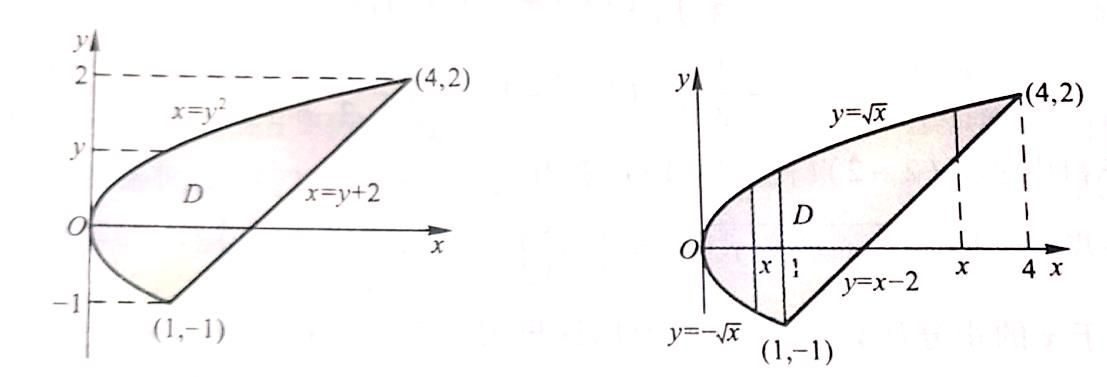
\includegraphics[scale=0.3]{Chapter 10 images/pic1.jpg}
    \]

    若利用公式\ref{10-2-1}来计算,则由于在区间$[0,1]$及$[1,4]$上表示$\varphi_1(x)$的式子不同,
    所以要用经过交点$(1,-1)$且平行于$y$轴的直线$x=1$把区域$D$分成$D_1$和$D_2$两部分(如图),其中
    
    $$
        \begin{aligned}
            & D_1=\left\{(x, y) \mid -\sqrt{x} \leq y \leq \sqrt{x}, 0 \leq x \leq 1 \right\} \\
            & D_2=\left\{(x, y) \mid x-2 \leq y \leq \sqrt{x}, 1 \leq x \leq 4 \right\}
        \end{aligned}
    $$

    因此,

    $$
        \begin{aligned}
            \iint_D x y \mathrm{~d} \sigma & =\iint_{D_1} x y \mathrm{~d} \sigma+\iint_{D_2} x y \mathrm{~d} \sigma \\
            & =\int_0^1\left[\int_{-\sqrt{x}}^{\sqrt{x}} x y \mathrm{~d} y\right] \mathrm{d} x+\int_1^4\left[\int_{x-2}^{\sqrt{x}} x y \mathrm{~d} y\right] \mathrm{d} x
        \end{aligned}
    $$

    \textbf{Problem 2}
    \vspace{1em}

    求两个底圆半径都等于\(R \)的直交圆柱面所围成的立体的体积。
    \vspace{1em}

    \textbf{Solution}
    \vspace{1em}

    设这两个圆柱面的方程分别为

    \[
        x^2+y^2=R^2 \text{及 } x^2+z^2=R^2
    \]

    利用立体关于坐标平面的对称性,只要算出它在第一卦限部分(图(a))的体积\(V_1\)再乘以\(8\)就行了。

    \[
        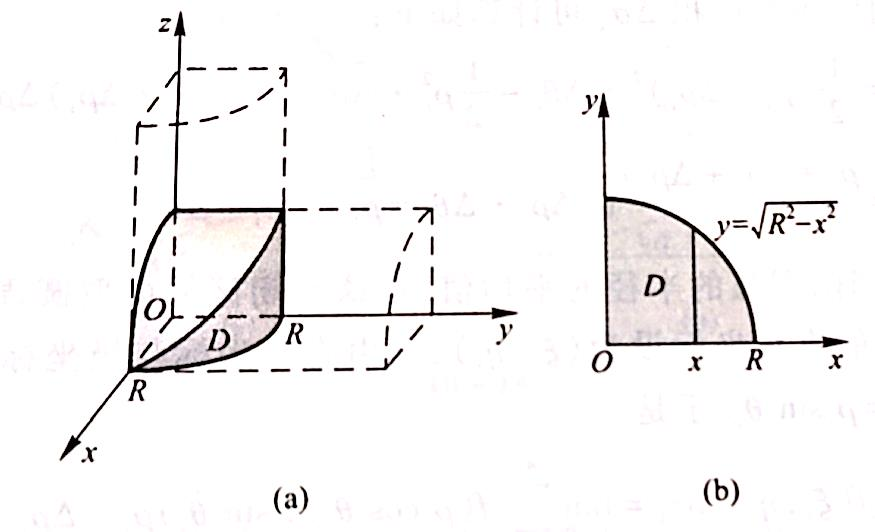
\includegraphics[scale=0.3]{Chapter 10 images/pic2.jpg}
    \]

    所求立体在第一卦限部分可以看成一个曲顶柱体,它的底为

    $$
        D=\left\{(x, y) \mid 0 \leq y \leq \sqrt{R^2-x^2}, 0 \leq x \leq R\right\}
    $$

    如图(b)所示。它的顶是柱面$z=\sqrt{R^2-x^2}$。于是

    $$
        V_1=\iint_D \sqrt{R^2-x^2} \mathrm{~d} \sigma
    $$

    所以

    $$
        \begin{aligned}
            V_1 & =\iint_D \sqrt{R^2-x^2} \mathrm{~d} \sigma \\
            & =\int_0^R\left[\int_0^{\sqrt{R^2-x^2}} \sqrt{R^2-x^2} \mathrm{~d} y\right] \mathrm{d} x \\
            & =\int_0^R\left[\sqrt{R^2-x^2} y\right]_0^{\sqrt{R^2-x^2}} \mathrm{~d} x \\
            & =\int_0^R\left(R^2-x^2\right) \mathrm{d} x \\
            & =\frac{2}{3} R^3
        \end{aligned}
    $$

    从而所求立体的体积为

    $$
        V=8 V_1=\frac{16}{3} R^3
    $$

\subsection{利用极坐标计算二重积分}

\subsubsection{二重积分的极坐标形式}

    $$
        \iint_D f(x, y) \mathrm{d} \sigma=\iint_D f(\rho \cos \theta, \rho \sin \theta) \rho \mathrm{d} \rho \mathrm{~d} \theta
    $$

    把极坐标上点\(\left(\rho, \theta\right)\)看作是在同一平面上的点\(\left(x,y\right)\)的极坐标表示,
    所以上式右端的积分区域仍然记作\(D \)。因为在直角坐标系中\({\displaystyle \iint_{D }f\left(x,y\right)\rmd \sigma}\)
    也常记作\({\displaystyle \iint_{D }f\left(x,y\right)\rmd x \rmd y}\),所以上式又可写成

    \begin{equation}
        \iint_D f(x, y) \mathrm{d} x \mathrm{~d} y=\iint_D f(\rho \cos \theta, \rho \sin \theta) \rho \mathrm{d} \rho \mathrm{~d} \theta
        \label{10-2-6}
    \end{equation}

\subsubsection{极坐标系下的二重积分化为二次积分}

    设积分区域$D$可以用不等式

    $$
        \varphi_1(\theta) \leq \rho \leq \varphi_2(\theta), \quad \alpha \leq \theta \leq \beta
    $$

    来表示,其中函数$\varphi_1(\theta)$、$\varphi_2(\theta)$在区间$[\alpha, \beta]$上连续。

    极坐标中二重积分化为二次积分的公式为

    \begin{equation}
        \iint_D f(\rho \cos \theta, \rho \sin \theta) \rho \mathrm{d} \rho \mathrm{~d} \theta=
        \int_\alpha^\beta\left[\int_{\varphi_1(\theta)}^{\varphi_2(\theta)} f(\rho \cos \theta, \rho \sin \theta) \rho \mathrm{d} \rho\right] \mathrm{d} \theta
    \end{equation}

    上式也写成

    \begin{equation}
        \iint_D f(\rho \cos \theta, \rho \sin \theta) \rho \mathrm{d} \rho \mathrm{~d} \theta=
        \int_\alpha^\beta \mathrm{d} \theta \int_{\varphi_1(\theta)}^{\varphi_2(\theta)} f(\rho \cos \theta, \rho \sin \theta) \rho \mathrm{d} \rho
        \label{10-2-8}
    \end{equation}

    如果积分区城$D$是如图所示的曲边扇形,那么可以把它看作当$\varphi_1(\theta) \equiv 0, \varphi_2(\theta)=\varphi(\theta)$\\
    时的特例,这时闭区域$D$可以用不等式

    \[
        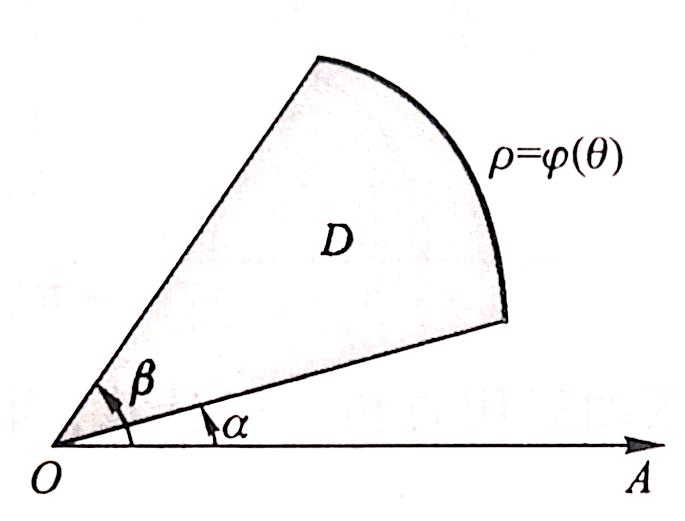
\includegraphics[scale=0.2]{Chapter 10 images/pic4.jpg}
    \]

    $$
        0 \leq \rho \leq \varphi(\theta), \alpha \leq \theta \leq \beta
    $$

    来表示,而公式\ref{10-2-8}成为

    $$
        \iint_D f(\rho \cos \theta, \rho \sin \theta) \rho \mathrm{d} \rho \mathrm{~d} \theta=
        \int_a^\theta \mathrm{d} \theta \int_0^{\varphi(\theta)} f(\rho \cos \theta, \rho \sin \theta) \rho \mathrm{d} \rho
    $$

    如果积分区城$D$如图所示,极点在\(D\)的内部,那么可以把它看作当$\alpha = 0, \beta = 2\uppi$
    时的特例,这时闭区域$D$可以用不等式

    \[
        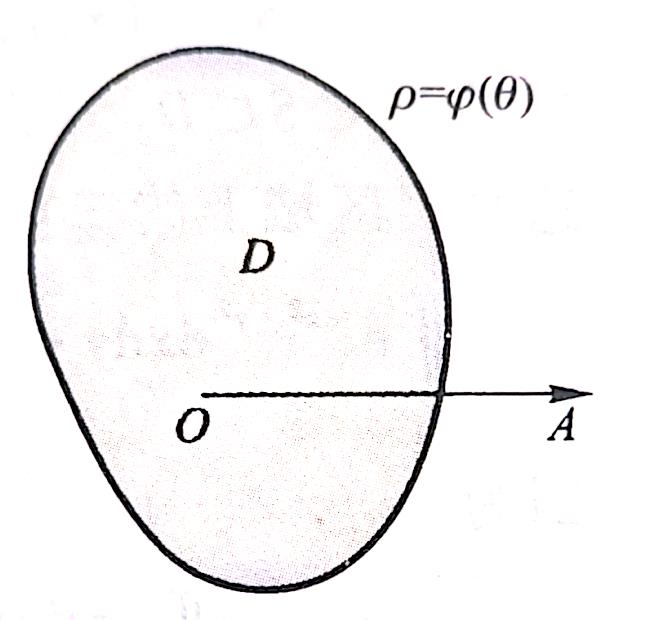
\includegraphics[scale=0.2]{Chapter 10 images/pic3.jpg}
    \]

    $$
        0 \leq \rho \leq \varphi(\theta), \quad 0 \leq \theta \leq 2 \uppi
    $$

    来表示,而公式\ref{10-2-8}成为

    $$
        \iint_D f(\rho \cos \theta, \rho \sin \theta) \rho \mathrm{d} \rho \mathrm{~d} \theta
        =\int_0^{2 \uppi} \mathrm{~d} \theta \int_0^{\varphi(\theta)} f(\rho \cos \theta, \rho \sin \theta) \rho \mathrm{d} \rho
    $$

    \textbf{注意}:

    \begin{enumerate}
        \item \({\displaystyle \sigma = \iint_D \rmd \sigma}\)表示闭区域\(D \)的面积;
        \item \({\displaystyle \sigma = \iint_D \rmd x \rmd y}\)表示直角坐标系中闭区域\(D \)的面积;
        \item \({\displaystyle \sigma = \iint_D \rho \rmd \rho \rmd \theta}\)表示极坐标系中闭区域\(D \)的面积;
    \end{enumerate}

    设积分区域$D$可以用不等式

    $$
        \varphi_1(\theta) \leq \rho \leq \varphi_2(\theta), \quad \alpha \leq \theta \leq \beta
    $$

    来表示,其中函数$\varphi_1(\theta)$、$\varphi_2(\theta)$在区间$[\alpha, \beta]$上连续,则有

    $$
        \sigma=\iint_D \rho \mathrm{~d} \rho \mathrm{~d} \theta=
        \int_\alpha^\beta \mathrm{d} \theta \int_{\varphi_1(\theta)}^{\varphi_2(\theta)} \rho \mathrm{d} \rho
        =\frac{1}{2} \int_\alpha^\beta\left[\varphi_2^2(\theta)-\varphi_1^2(\theta)\right] \mathrm{d} \theta
    $$

    如果积分区城$D$是曲边扇形,那么可以把它看作当$\varphi_1(\theta) \equiv 0, \varphi_2(\theta)=\varphi(\theta)$
    时的特例,这时有

    $$
        \sigma=\frac{1}{2} \int_\alpha^\beta \varphi^2(\theta) \mathrm{d} \theta
    $$

\subsubsection{例题}

    \textbf{Problem 1}
    \vspace{1em}

    计算${\displaystyle \iint_D e^{-x^2-y^2} \rmd x \rmd y}$,其中$D$是由圆心在原点、半径为\(a \)的圆周所围成的闭区域。
    \vspace{1em}

    \textbf{Solution}
    \vspace{1em}

    在极坐标系中,闭区域\(D \)可表示为

    \[
        0 \leq \rho \leq a, 0 \leq \theta \leq 2 \uppi
    \]

    于是有

    $$
        \begin{aligned}
            \iint_D \mathrm{e}^{-x^2-y^2} \mathrm{~d} x \mathrm{~d} y & =\iint_D \mathrm{e}^{-\rho^2} \rho \mathrm{~d} \rho \mathrm{~d} \theta=\int_0^{2 \uppi}\left[\int_0^a \mathrm{e}^{-\rho^2} \rho \mathrm{~d} \rho\right] \mathrm{d} \theta \\
            & =\int_0^{2 \uppi}\left[-\frac{1}{2} \mathrm{e}^{-\rho^2}\right]_0^a \mathrm{~d} \theta=\frac{1}{2}\left(1-\mathrm{e}^{-a^2}\right) \int_0^{2 \uppi} \mathrm{~d} \theta \\
            & =\uppi\left(1-\mathrm{e}^{-a^2}\right)
        \end{aligned}
    $$
    \vspace{1em}

    利用上面的结果计算反常积分\({\displaystyle \int_{0}^{+\infty} e^{-x^2} \rmd x}\):

    设

    $$
        D_1=\left\{(x, y) \mid x^2+y^2 \leq R^2, x \geq 0, y \geq 0\right\}
    $$

    $$
        D_2=\left\{(x, y) \mid x^2+y^2 \leq 2 R^2, x \geq 0, y \geq 0\right\}
    $$

    $$
        S=\{(x, y) \mid 0 \leq x \leq R, 0 \leq y \leq R\}
    $$

    \[
        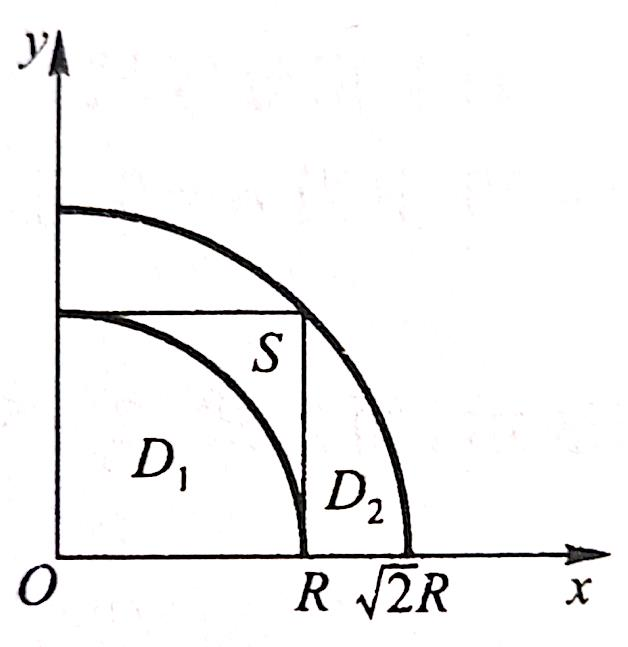
\includegraphics[scale=0.2]{Chapter 10 images/pic5.jpg}
    \]

    显然\(D_1 \subset S \subset D_2\)。由于\(e^{-x^2-y^2} > 0\),从而在这些闭区域上的二重积分之间有不等式

    $$
        \iint_{D_1} \mathrm{e}^{-x^2-y^2} \mathrm{~d} x \mathrm{~d} y<
        \iint_S \mathrm{e}^{-x^2-y^2} \mathrm{~d} x \mathrm{~d} y<\iint_{D_2} \mathrm{e}^{-x^2-y^2} \mathrm{~d} x \mathrm{~d} y
    $$

    因为

    $$
        \iint_S \mathrm{e}^{-x^2-y^2} \mathrm{~d} x \mathrm{~d} y=
        \int_0^R \mathrm{e}^{-x^2} \mathrm{~d} x \cdot \int_0^R \mathrm{e}^{-y^2} \mathrm{~d} y
        =\left(\int_0^R \mathrm{e}^{-x^2} \mathrm{~d} x\right)^2
    $$

    又应用上面已得的结果有

    $$
        \iint_{D_1} \mathrm{e}^{-x^2-y^2} \mathrm{~d} x \mathrm{~d} y=\frac{\uppi}{4}\left(1-\mathrm{e}^{-R^2}\right)
    $$

    $$
        \iint_{D_2} \mathrm{e}^{-x^2-y^2} \mathrm{~d} x \mathrm{~d} y=\frac{\uppi}{4}\left(1-\mathrm{e}^{-2 R^2}\right)
    $$

    于是上面的不等式可以写成

    $$
        \frac{\uppi}{4}\left(1-\mathrm{e}^{-R^2}\right)<\left(\int_0^R \mathrm{e}^{-x^2} \mathrm{~d} x\right)^2<\frac{\uppi}{4}\left(1-\mathrm{e}^{-2 R^2}\right)
    $$

    令\(R \rightarrow +\infty\),上式两端趋于同一极限\(\frac{\uppi}{4}\),从而

    $$
        \int_0^{+\infty} e^{-x^2} d x=\frac{\sqrt{\uppi}}{2}
    $$
    \vspace{1em}

    \textbf{Problem 2}
    \vspace{1em}

    求球体\(x^2+y^2+z^2 \leq 4a^2\)被圆柱面\(x^2+y^2=2ax,\; (a>0)\)所截得的(含在圆柱面内的部分)立体的体积。

    \[
        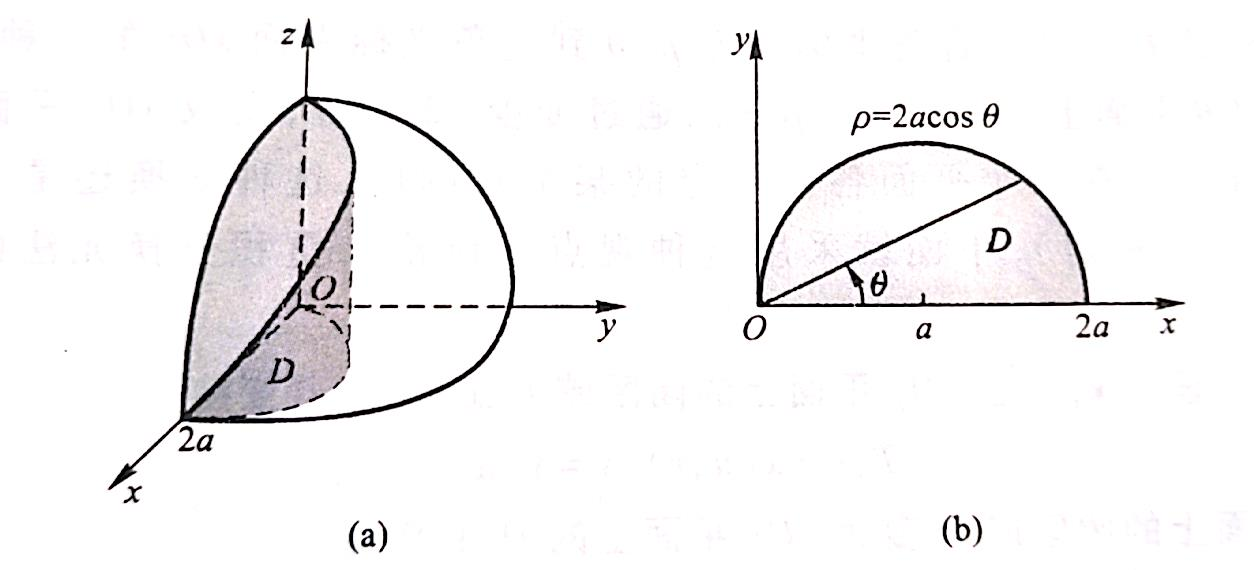
\includegraphics[scale=0.2]{Chapter 10 images/pic6.jpg}
    \]
    \vspace{1em}

    \textbf{Solution}
    \vspace{1em}

    由对称性

    $$
        V=4 \iint_D \sqrt{4 a^2-x^2-y^2} \mathrm{~d} x \mathrm{~d} y,
    $$

    其中\(D \)为半圆周\(y=\sqrt{2ax-x^2}\)及\(x \)轴所围成的闭区域。在极坐标系中,闭区域\(D \)可用不等式

    $$
        0 \leq \rho \leq 2 a \cos \theta, \quad 0 \leq \theta \leq \frac{\uppi}{2}
    $$

    来表示。于是

        $$
        \begin{aligned}
            V & =4 \iint_D \sqrt{4 a^2-\rho^2} \rho \mathrm{~d} \rho \mathrm{~d} \theta=4 \int_0^{\frac{\uppi}{2}} \mathrm{~d} \theta \int_0^{2 a \cos \theta} \sqrt{4 a^2-\rho^2} \rho \mathrm{~d} \rho \\
            & =\frac{32}{3} a^3 \int_0^{\frac{\uppi}{2}}\left(1-\sin ^3 \theta\right) \mathrm{d} \theta=\frac{32}{3} a^3\left(\frac{\uppi}{2}-\frac{2}{3}\right)
        \end{aligned}
    $$

\end{document}
